\documentclass{beamer}
\usepackage[utf8]{inputenc}
% \usepackage[english]{babel}
\usepackage{hyperref}
\usepackage{graphicx}
\graphicspath{{../../../output/figures/Presentation/}}
\usepackage{wrapfig}
\usepackage{subcaption}
\usepackage{booktabs,bbm}
\usepackage[space]{grffile}
% \usepackage[square,numbers]{natbib}
%\bibliographystyle{unsrtnat}

\makeatletter
\let\@@magyar@captionfix\relax
\makeatother
\newtheorem{defn}[theorem]{Definition}
\DeclareMathOperator*{\argmax}{arg\,max}
\DeclareMathOperator*{\argmin}{arg\,min}
\hypersetup{
    allcolors={}
}

\usetheme{Boadilla}
\usecolortheme{beaver}

\usepackage[
backend=biber,
style=bwl-FU,
sorting=ynt
]{biblatex}
\addbibresource{../../main.bib}

\title[Agricultural Index Insurance]{Agricultural Index Insurance: An Optimization Approach}
\author[José Velarde Morales]{José I. Velarde Morales \and Linwei Xin}
\institute[Chicago Booth]
{

  University of Chicago\\
  Booth School of Business

}


\begin{document}
\beamertemplatenavigationsymbolsempty
\frame{\titlepage}
\section{Introduction}

% \subsection*{The Problem of Agricultural Risk}
% \begin{frame}{The Problem of Agricultural Risk}
% \begin{itemize}
%     \setlength\itemsep{2em}
%     \item Farmers face a lot of risk, and the lack of risk management tools forces them to use coping strategies that hurt their long term welfare.
   
%     \item Traditional insurance is prohibitively costly in most developing countries due to lack of data and high verification costs.

%     \item Moral hazard, adverse selection, and the presence of large covariate shocks make the problem of agricultural insurance especially hard. 
% \end{itemize}
% \end{frame}

% \subsection*{A Proposed Solution: Index Insurance}
% \begin{frame}{A Proposed Solution: Index Insurance}
% \begin{itemize}
%    \setlength\itemsep{1em}
%     % \item Researchers developed index insurance as a less costly way to offer insurance in developing countries. 
%     \item In index insurance, an index (or statistic) is created using easily observable quantities (e.g. rainfall), and it is used to determine whether the insured party suffered an adverse event. 
%     \item If the index falls below a pre-determined threshold, the insurance company automatically issues out payments to the insured. 
%     \item This allows the insurance company to circumvent the issue of verification and moral hazard, since the actions of individual farmers cannot affect the index.
% \end{itemize}
% \end{frame}

\subsection*{Project Overview}
\begin{frame}{Project Overview}
 \begin{itemize}
    \setlength\itemsep{1em}   
    % \item Traditionally, contracts are designed to maximize correlation between payouts and losses (\cite{chantarat2013designing}).  %This ignores valuable information about the correlation between zones that affects the cost of insuring the whole portfolio. 
    \item The goal of this project is to improve the design of index insurance contracts. I am particularly interested in the developing country setting.  
    \item The original motivation was to develop a method to simultaneously design contracts for all insured zones, in order to better manage risk. However, upon learning more about the context I realized that the optimization based approach could be an improvement even in the single zone case. 
    \item We develop a method that tries to maximize farmer utility, incorporates different kinds of constraints, and yields interpretable contracts. 
    % \item Our method simultaneously determines the contract parameters for different areas, while taking into account the correlation between the areas, reducing risk for the insurer. 
 \end{itemize}
\end{frame}

\begin{frame}{Motivation for multi-zone optimization}
    \begin{itemize}
        \item For the insurer, the risk (and therefor cost) of providing a line of insurance depends on the other lines of insurance in its portfolio. 
        \item If all of its lines of insurance are highly correlated, it will be more expensive due to capital requirements. 
        \item This is similar to the problem of portfolio design, where the correlations between stocks affect optimal portfolio composition. 
        \item Insurers can influence the composition of their portfolio through the contracts they offer, so they should be better able to manage
        their costs if they take into account the correlation of different lines of insurance when designing contracts.
    \end{itemize}
    
\end{frame}

\section{Background}
\begin{frame}[noframenumbering, plain]
    \frametitle{Content}
    \tableofcontents[currentsection]
  \end{frame}
\subsection{Index Insurance Background}
\begin{frame}{Index Insurance: Definition and Parameters}
    \begin{itemize}
        \setlength\itemsep{1em}
        \item Index insurance uses a signal, $\theta$, to predict agricultural loss, $\hat{\ell}(\theta)$
        \item Contract form: $I(\theta) = \min \left \{ \max \left \{a\hat{\ell}(\theta) - b,0 \right \}, 1 \right \}$, $a,b$ are the contract parameters.
        % \item Expected cost for insurer: $C(I(\theta)) = \mathbb{E}[I(\theta)] + c_{\kappa} K(I(\theta))$, where $c_{\kappa}$ is the cost of capital, and $K$ is required capital.
        % \item $K(I(\theta)) = CVaR_{1-\epsilon_P}\left ( I(\theta) \right ) - \mathbb{E}[I(\theta)]$.
    \end{itemize}
    \end{frame}
    
    \begin{frame}{Example of Index Insurance Contract}
        \begin{figure}
            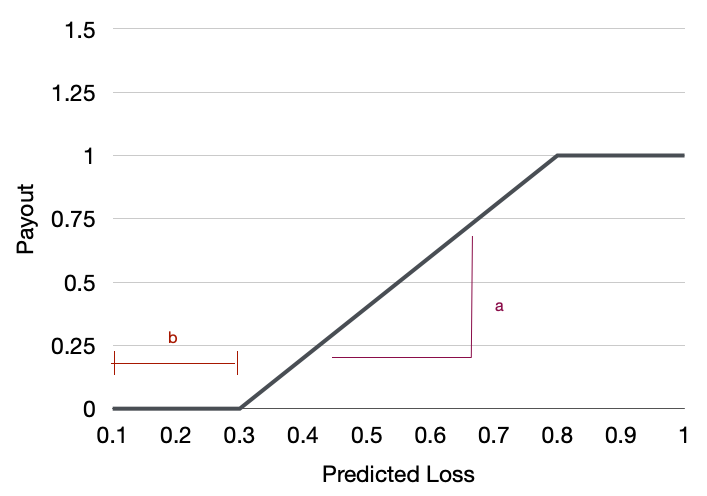
\includegraphics[width=0.9\textwidth]{../../../output/figures/Presentation/sample_insurance_contract.png}
        \end{figure}
    \end{frame}

\subsection{Current Approaches}
\begin{frame}{Current methods to design index insurance}
\begin{itemize}
    \setlength\itemsep{1em}
    \item \textbf{Baseline Method:} Predict then design, design contracts to maximize correlation between payouts and losses. \cite{chantarat2013designing}
    \begin{itemize}
        \item \textbf{Pros:} simple, interpretable
        \item \textbf{Cons:} can't incorporate constraints
    \end{itemize}
    \item \textbf{NN Based Method:} End to end, use NN to design contracts. Combine prediction and contract design into single step. \cite{chen2023managing}
    \begin{itemize}
        \item \textbf{Pros:} directly maximizes utility, admits price contstraints
        \item \textbf{Cons:} not interpretable, hard to adjust, requires a lot of data to train. 
    \end{itemize}
\end{itemize}
\end{frame} 

% \begin{frame}{Drawbacks of current methods}
%     \begin{itemize}
%         \setlength\itemsep{1em}
%         \item \textbf{Baseline Method:} 
%         \begin{itemize}
%             \item Can't incorporate constraints
%             \item Only adjusts one contract parameter
%         \end{itemize}
%         \item \textbf{NN Based Method:} 
%         \begin{itemize}
%             \item Not interpretable, can't set constraints on variables that policy makers might care about (e.g. deductible). This also makes it hard to debug: is the performance due to poor prediction performance? Too high a deductible? 
%             \item Requires a lot of data to train (model has 10,000 parameters)
%             \item Premium definition used only considers expected value of payouts. In practice, variance is highly important. 
%         \end{itemize}
%     \end{itemize}
%     \end{frame} 

\section{Optimization Approach}
\begin{frame}[noframenumbering, plain]
    \frametitle{Content}
    \tableofcontents[currentsection]
  \end{frame}
\subsection{Prediction}
\begin{frame}{Overview}
    \begin{itemize}
        \setlength\itemsep{2em}
        \item We opt for a "predict-then-optimize" approach.
        \item We use specialized time-series feature extraction algorithms and traditional ML algorithms (e.g. Random Forest, Gradient Boosting, Support Vector Machines) to build a loss prediction model.
        \item We then use model predictions and actual losses to design contracts to maximize utility. 
    \end{itemize}
\end{frame}

\begin{frame}{Our Method Flowchart}
    \begin{figure}
        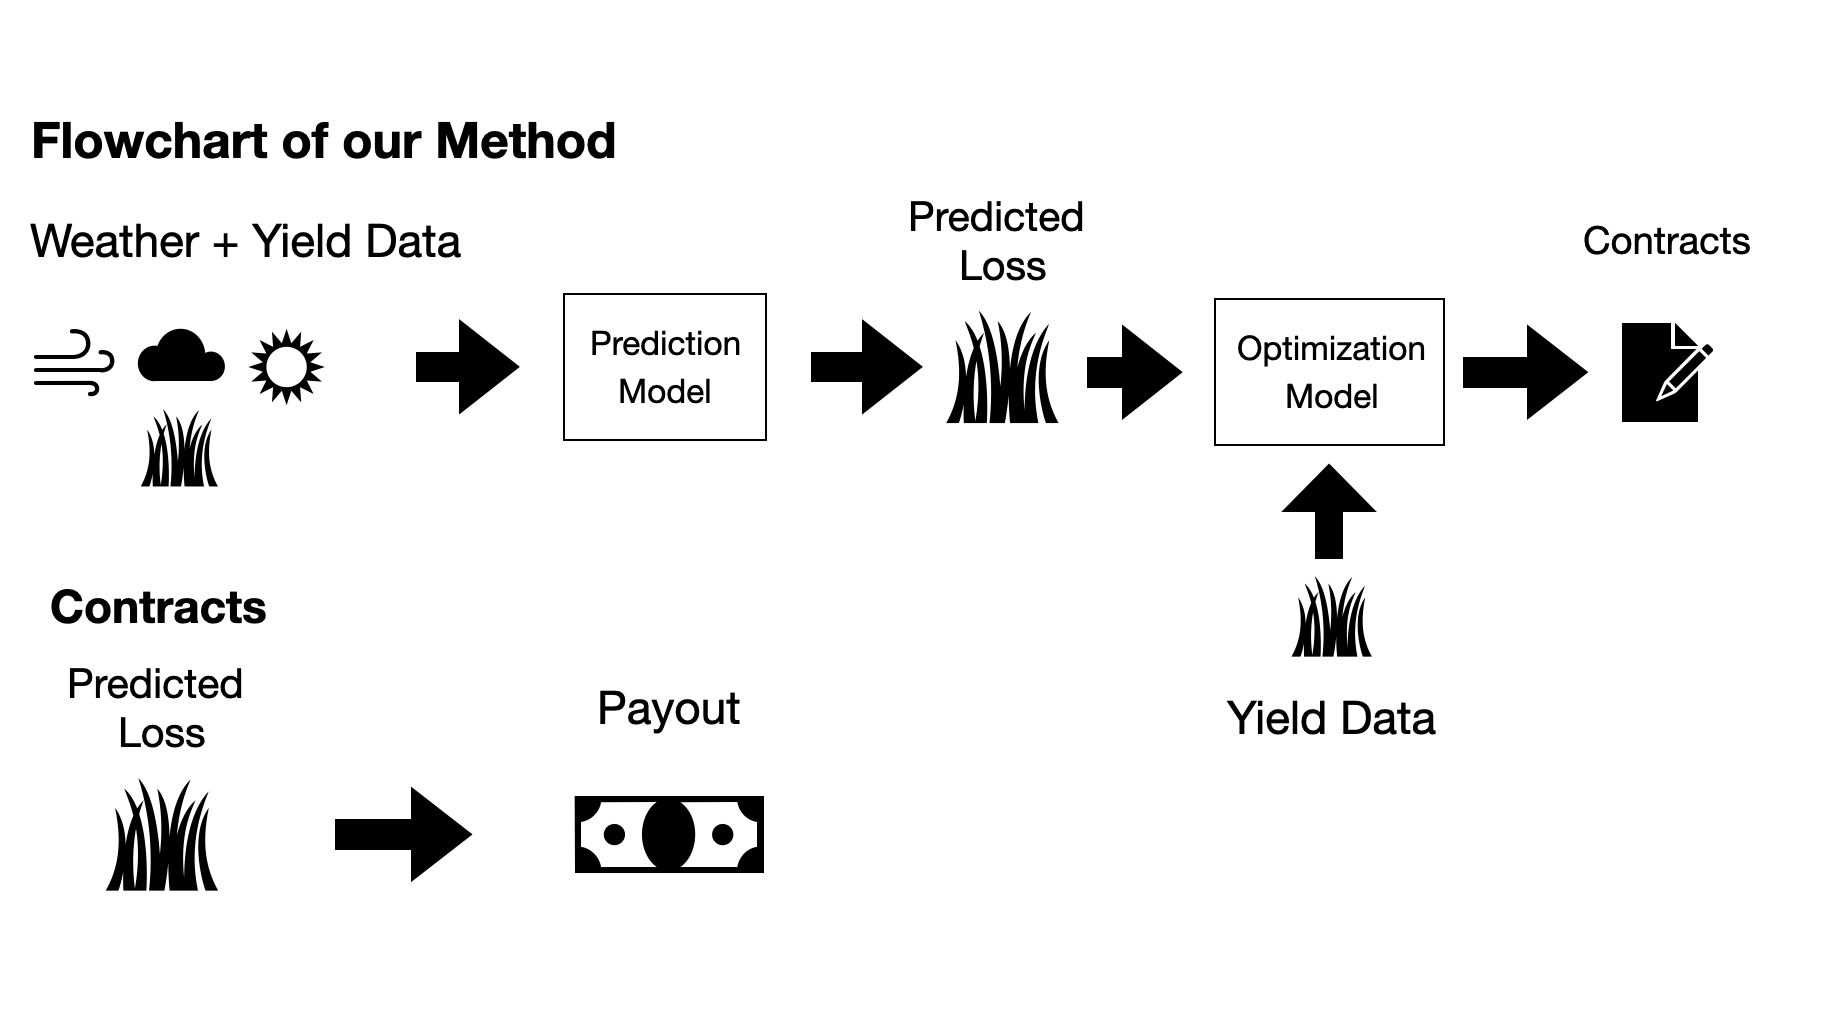
\includegraphics[width=\textwidth]{../../../output/figures/Our Method Flowchart.png}
    \end{figure}
\end{frame}

\begin{frame}{Benefits of Our Approach}
    \begin{itemize}
        \setlength\itemsep{2em}
        \item Can admit many common definitions of the premium
        \item Can incorporate price and payout frequency constraints
        \item Requires less data to train than NN approach. 
    \end{itemize}
\end{frame}

\subsection{Model}
\begin{frame}{Utility Framework/Model}
    \begin{align*}
        w &= w_0 + 1 - \ell + I(\hat{\ell}) - \pi\\
        \pi &= \mathbb{E}[I(\hat{\ell})] + c_{\kappa}K \\
        K &= \textsf{CVaR}_{1-\epsilon} \left ( I(\hat{\ell})  \right ) - \mathbb{E}[I(\hat{\ell})]
    \end{align*}

    CRRA Utility function: $u(w) = \frac{1}{1-\alpha} w^{1-\alpha}$.
    Premium definition comes from \textit{Risk Modeling for Appraising Named Peril Index Insurance Products: A Guide for Practitioners} (\cite{mapfumo2017risk}). The EU's Solvency requirements are similar.

\end{frame}

% \begin{frame}{Premium Principles}
%     Premium principles are the functionals used to map insurance contracts to premiums (prices). The exact pricing method used by insurers is considered to be proprietary information. However, there are several premium principles that are common in the actuarial literature, and our method is compatible with most of them:
%     \begin{table}[h!]
%         \centering
%         \begin{tabular}{ll}
%         Description & Definition \\ \hline
%         Expected value       & $(1+\alpha)\mathbb{E}[I]$           \\
%         Standard deviation   & $\mathbb{E}[I] + \alpha \sigma(I)$       \\
%         Variance             & $\mathbb{E}[I] + \alpha \sigma^2(I)$      \\
%         Exponential          & $\frac{1}{\alpha} \log \mathbb{E}[e^{\alpha I}]$    \\
%         Dutch                &  $\mathbb{E}[I] + \beta \mathbb{E}[(I-\alpha \mathbb{E}[I])_+]$                   \\ \hline
%         \end{tabular}
%         \end{table}
% \end{frame}


\begin{frame}{Idealized Model}
\begin{align}
    \max_{a,b,\pi, K}  & \quad \mathbb{E} \left [ U\left ( w_0 - \ell - \pi + I(\theta) \right ) \right ] \label{cons-objective}\\
    \text{s.t.} & \quad I(\theta) =  \min \left \{\max \left \{0,a\hat{\ell}(\theta) + b \right \}, 1 \right \}\label{cons-contract}\\
    & \quad \pi = \mathbb{E}\left [ I(\theta) \right ] + c_{\kappa} \left[ {\sf CVaR}_{1-\epsilon_K}\left ( I(\theta)\right )  - \mathbb{E}[I(\theta)]  \right] \\
    % & \quad \underline{f} \leq \mathbb{P}\left ( I(\theta) > 0 \right ) \leq \overline{f} \label{cons-frequency}\\
    &\quad \pi \leq \overline{\pi}.
\end{align}
\end{frame}


\begin{frame}{Convex Relaxation}
    \begin{align}
        \max_{a,b,K,\pi} &\quad \mathbb{E} \left [  U\left(w_0 - \ell - \pi  +  \underline{I(\theta)} \right) \right ]\label{eq-06}\\
        \text{s.t.} & \quad \overline{I(\theta)} = \max \left \{0,a\hat{\ell}(\theta) + b \right \} \nonumber\\
        & \quad \underline{I(\theta)} = \min \left \{a\hat{\ell}(\theta)+b,1 \right \} \nonumber\\
        & \quad \pi = \left (1-c_{\kappa} \right ) \mathbb{E} \left [ \overline{I(\theta)} \right ] + c_{\kappa} {\sf CVaR}_{1-\epsilon_K} \left( \overline{I(\theta)} \right) \label{eq-41}\\
        % & \quad a \hat{F}^{-1}(\overline{f}) \leq b \leq a\hat{F}^{-1}(\underline{f})\\
        & \quad \pi \leq \overline{\pi} \nonumber.
  \end{align}
    
\end{frame}

\begin{frame}{Multiple Zone Case}
    In the multi-zone case, the problems are coupled through the required capital
    \begin{align*}
        K &= \textsf{CVaR}_{1-\epsilon} \left ( \sum_z s_z I_z(\hat{\ell_z}) \right ) - \mathbb{E}\left [\sum_z s_z I_z(\hat{\ell_z}) \right ]
    \end{align*}

    The first term will be affected by the correlation of losses across zones, so the optimal contracts will vary depending on this correlation. 
    
\end{frame}

\begin{frame}{Multiple Zone Model}
    \begin{align}
        \max_{a,b,K,\pi} &\quad \mathbb{E}\left [ \sum_z U\left ( w_{0,z} -\ell_z^j -\pi_z + I_z(\theta^j_z) \right ) \right ]\label{eq-33}\\
        \text{s.t.} &\quad \pi_z  = \mathbb{E}\left [ \overline{I_z(\theta_z)} \right ] + \frac{c_{\kappa}}{\sum_z s_z}  K\\
        &\quad K = {\sf CVaR}_{1-\epsilon_K} \left ( \sum_z s_z\overline{I_z(\theta_z)} \right ) - \mathbb{E}\left [ \sum_{z} s_{z}\underline{I_{z}(\theta_{z'})} \right ] \label{eq-32}\\
        % & \quad a_z\hat{\ell_{z}^{\underline{f}}} \leq b_z \leq a_z\hat{\ell_{z}^{\overline{f}}}\\
        &\quad \overline{I_z(\theta_z)} = \max \left \{0,a_z\hat{\ell_z}(\theta_z) + b_z \right \} \nonumber\\
        &\quad\underline{I_z(\theta_z)} = \min \left \{a_z\hat{\ell_z}(\theta_z)+b_z,1 \right \} \nonumber\\
        &\quad\pi_z \leq \overline{\pi_z} \nonumber.
      \end{align}
\end{frame}

\section{Evaluation: Thai Data}
\begin{frame}[noframenumbering, plain]
    \frametitle{Content}
    \tableofcontents[currentsection]
  \end{frame}

\begin{frame}{Evaluation: Thai Data}
    \begin{itemize}
        \setlength \itemsep{2em}
        \item Index isurance is especially popular in developing countries beacuse of its low cost.
        \item However, one of the difficulties in studying index insurance is the lack of data in these settings. 
        \item I collaborated with the Bank of Thailand and was given access to a novel dataset of census-tract-level (Tambon) losses from natural disasters.
    \end{itemize}
    
\end{frame}
\subsection{Data}
\begin{frame}{Thai Data: Administrative Data Sources}
    \begin{itemize}
        \setlength\itemsep{2em}
        \item Thailand Department of Agricultural Extension (DOAE): This dataset contains detailed information on the planting activities of over 3.1 million Thai farmers. Information includes plant date, plot size, rice variety, etc
        \item Thai Governemnt Disaster Relief Data: This data is from the current national disaster relief program. It contains information about the disaster type, losses, and disaster date.  
    \end{itemize}
\end{frame}

\begin{frame}{Remote Sensing Data Sources}
    \begin{itemize}
        \setlength\itemsep{2em}
        \item Climate Hazards Center InfraRed Precipitation with Station data (CHIRPS): daily rainfall data 1981-present
        \item MOD21A1 Land Surface Temperature: daily temperature data, available 2000-present 
        \item FLDAS Famine Early Warning Systems Network: monthly evapotranspiration data, available 1992-present
    \end{itemize}
\end{frame}

\begin{frame}{Data Summary Statistics}
    \begin{figure}[h]
        \centering
        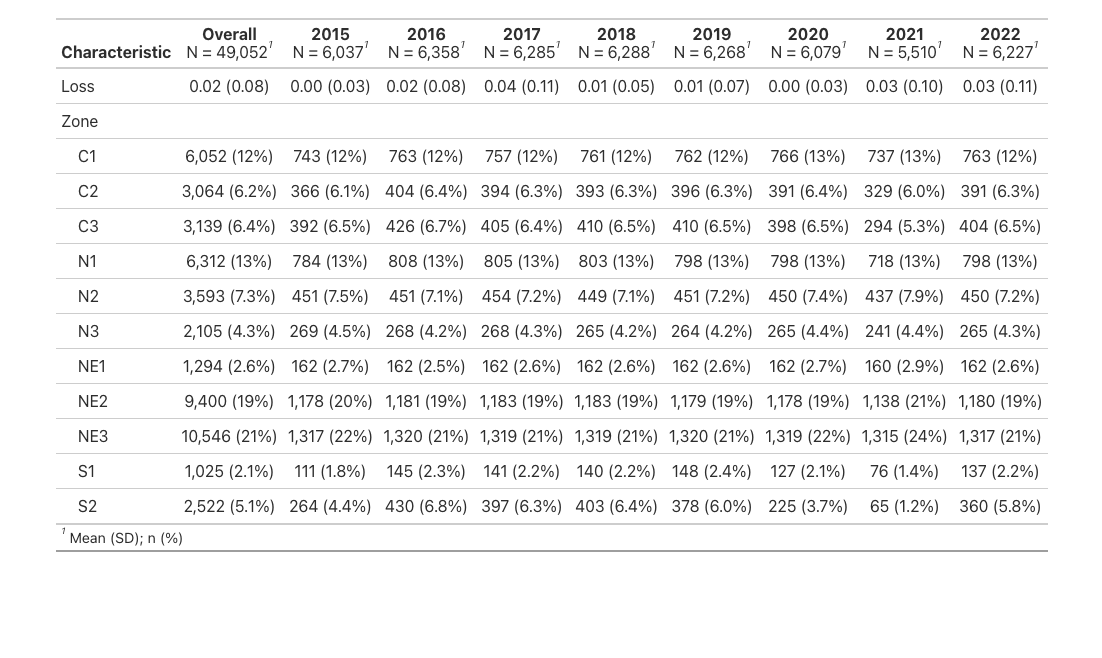
\includegraphics[width=\textwidth]{thai_summary_stats.png}
    \end{figure}
\end{frame}

\begin{frame}{Disaster Activity Map}
    \begin{figure}[h]
        \centering
        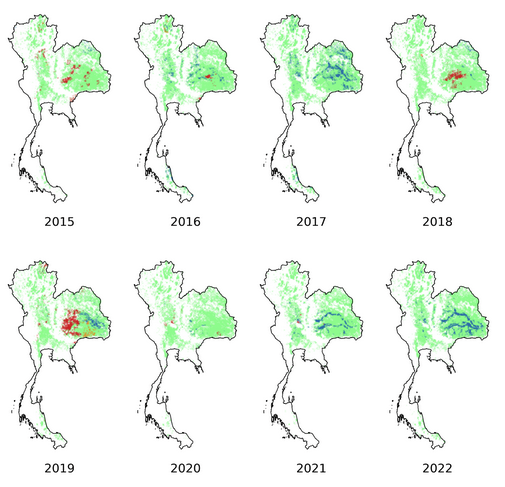
\includegraphics[width=0.6\textwidth]{disaster_map.png}
    \end{figure}
\end{frame}

\subsection{Procedure}
\begin{frame}{Evaluation Procedure}
    \begin{itemize}
        \setlength\itemsep{2em}
        \item We use leave one year out cross validation. 
        \item In each CV fold, data from year $y$ is used for testing. Data from $y'\neq y$ is used for insurance design (prediction model training and contract design).
        \item This gives us out of sample predictions for every observation in our data. We then compute utility-based performance metrics across all out of sample predictions. 
    \end{itemize}
\end{frame}

\begin{frame}{Evaluation Details}
    \begin{itemize}
        \item We use training data to compute premium $\rightarrow$ this reflects practice.
        \item We modify Chen's method to use the same premium definition as ours. 
        \item We use a copula approach to estimate the $\textsf{CVaR}$ when calculating the premium. 
        \item Same method is used to calculate the premium for all methods. 
        \item We use a CRRA utility function with $\alpha=1.5$. 
    \end{itemize}
    
\end{frame}

\subsection{Framework}
\begin{frame}{Perfromance Metrics}
    We focus on the Relative Insurance Benefit (RIB) (\cite{kenduiywo2021evaluating}) as a performance metric. It measures the share of all possible welfare gains that are recovered by our insurance. \\
    \begin{itemize}
        \setlength\itemsep{1em}
        \item Relative Insurance Benefit (RIB): $\frac{CE^J - CE^{NI}}{CE^{PI}-CE^{NI}}$
        \item Certainty equivalent (CE): $u^{-1}(\mathbb{E}[u(w^I)])$
        \item Utility: $u(w) = \frac{1}{1-\alpha} w^{\frac{1}{1-\alpha}}$
    \end{itemize}
\end{frame}

\subsection{Single Zone Results}
\begin{frame}{Results for $c_k=0.02, \alpha=1.5$ }
    Here, the contract design and pricing for each zone happens independently of all other zones. 
    \begin{table}[]
        \centering
        \small
        \caption{Single Zone Results}
        \begin{tabular}{llllll}
        \textbf{Method} & \textbf{RIB}  & \textbf{Premium} & \textbf{Cost II} & \textbf{Cost PI} & \textbf{CapShare} \\
        VMX       & 0.874   & 0.022 & 0.028 & 0.030 & 0.125 \\
        Chantarat & -0.249  & 0.005 & 0.003 & 0.030 & 0.227 \\
        Chen      & -8.797  & 0.096 & 0.061 & 0.030 & 0.257
        \end{tabular}
        \end{table}
    
\end{frame}

\begin{frame}{Single Zone Results Key Points}
    \begin{itemize}
        \setlength\itemsep{2em}
        \item Our method achieves $67\%$ of the utility gains of perfect insurance. 
        \item Has a lower percentage of the premium cost going to required capital. 
    \end{itemize}
\end{frame}

\begin{frame}{Note on the value of $c_{\kappa}$}
    \begin{itemize}
        \item Potential value for farmers is highly dependent on $c_{\kappa}$ and risk aversion, $\alpha$
        \item For the most commonly used value of $\alpha$, farmers could only benefit from perfect insurane if $c_{\kappa}=0.02$.
        \item As risk aversion increases, the gains from perfect insurance increase. 
    \end{itemize}
\end{frame}

\begin{frame}{Effects of Cost of Capital and Risk Aversion}
    \begin{figure}
        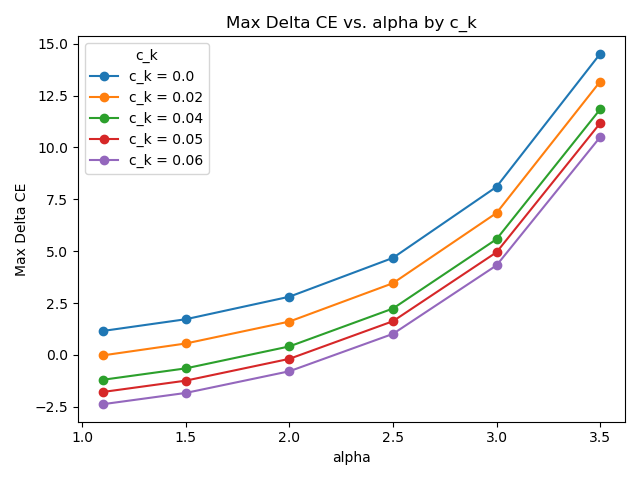
\includegraphics[width=0.75\textwidth]{../../../output/figures/Feedback/MaxDeltaCE.png}
        \caption{Perfect Insurance}
    \end{figure}
    
\end{frame}


\begin{frame}{Multi zone results}
    \begin{itemize} 
        \item Multi zone model performs worse than just optimizing contract for each zone independently :(
    \end{itemize}
    
\end{frame}

\section{US Midwest Evaluation}
\begin{frame}[noframenumbering, plain]
    \frametitle{Content}
    \tableofcontents[currentsection]
  \end{frame}
\subsection{Data}
\begin{frame}{Data}
    Used two main data sources
    \begin{itemize}
        \setlength\itemsep{2em}
        \item Illinois annual corn yield data from the National Agricultural Statistics Service (NASS). Data is available at the county level from 1925-2022. 84 counties. 
        \item Weather data from the PRISM climate group. Has monthly data on several weather variables (temperature, precipitation, etc). Available 1895-present.
    \end{itemize}
\end{frame}

\subsection{Procedure}
\begin{frame}{Evaluation Procedure}
    \begin{itemize}
        \setlength\itemsep{2em}
        \item We use a 70/15/15 train/val/test split. Data is kept in chronological order. Training data has older years and test data has the newest years. 
        \item We modified Chen's method to use the same definition of the premium as our method. 
        \item We use the training and validation data to design the contracts using both methods, apply the contracts to farmers in the test set, and compute performance metrics. 
        \item We used a data shortening exercise to evaluate how the performance of both methods changed as more data became available. 
    \end{itemize}
\end{frame}


\subsection{Illinois Results}
\begin{frame}{Overview}
    \begin{itemize}
        \setlength\itemsep{2em}
        \item Our method performs similarly or outperforms the Chen model when there is less than 50 years of data available.  
        \item In terms of farmer utility, our method tends to work better with realistic data lengths. Most satellite data starts at 1980 at the earliest. 
        \item When using data from other states, our method consistently outperforms Chen's method, but is not always better than no insurance, at least at the full premium price. This might not be a huge problem, since agricultural insurance tends to be heavily subsidized, both in rich and poor countries. In the US, it averaged $62\%$ of premiums in 2022. 
    \end{itemize}
\end{frame}

% \begin{frame}{Illinois: Utility}
%     \begin{figure}
%         % 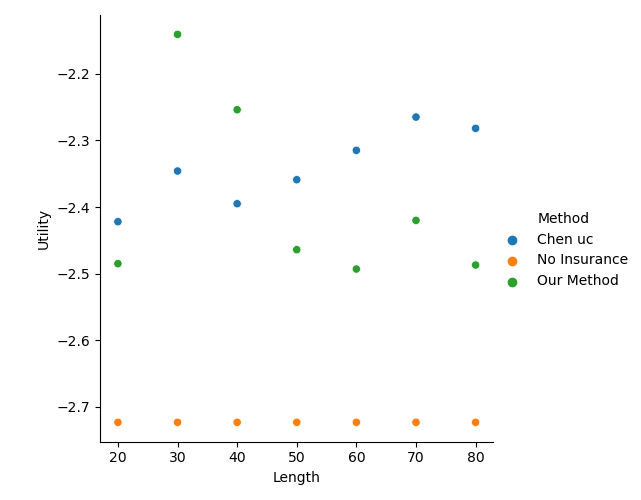
\includegraphics[width=0.75\textwidth]{../../../output/figures/Evaluation 2/Illinois_Utility_Length_ml1.png}
%         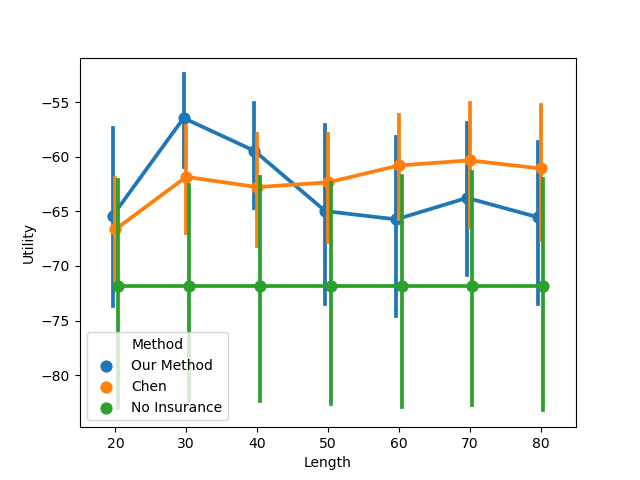
\includegraphics[width=0.75\textwidth]{../../../output/figures/Evaluation/Illinois_Average_Utility_CI.png}
%     \end{figure}
% \end{frame}

\begin{frame}{Illinois Short Data (Less than 40 years)}
    \begin{table}
        \centering
        \begin{tabular}{lrrr}
            \toprule
            Method & DeltaCE & Premium & Required Capital \\
            \midrule
            Chantarat & 4.13 & 113.96 & 158.73 \\
            Chen uc & 4.87 & 60.69 & 134.35 \\
            Our Method & 5.31 & 62.49 & 97.91 \\
            \bottomrule
            \end{tabular}
    \end{table}
    
        
\end{frame}

\begin{frame}{Illinois Long Data (More than 40 years)}
    \begin{table}
        \centering
        \begin{tabular}{lrrr}
            \toprule
            Method & DeltaCE & Premium & Required Capital \\
            \midrule
            Chantarat & 2.05 & 105.53 & 135.72 \\
            Chen uc & 4.82 & 50.06 & 115.02 \\
            Our Method & 3.82 & 41.75 & 67.80 \\
            \bottomrule
            \end{tabular}
    \end{table}
    
\end{frame}

% \begin{frame}{Illinois: Insurer Cost}
%     \begin{figure}
%         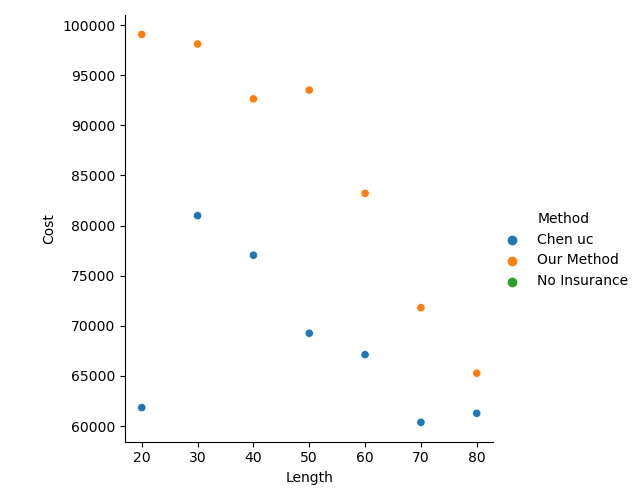
\includegraphics[width=0.75\textwidth]{../../../output/figures/Evaluation/Illinois_Cost_Length_ml1.png}

%     \end{figure}
% \end{frame}




% \subsection{Insuring the US Midwest}
% \begin{frame}[noframenumbering, plain]
%     \frametitle{Content}
%     \tableofcontents[currentsubsection]
%   \end{frame}


\subsection{Multi zone Results}
\begin{frame}{Overview}
    \begin{itemize}
        \item Our multiple zone model adjusts contracts based on the correlation between the insured zones. In this case, it leads to contracts that pay out more frequently, but at a lower rate. This reduces the tail risk for the insurer and reduces the amount of capital needed. 
        \item It outperforms Chen's model and the no insurance case consistently, and has lower costs and required capital than the Chen model. 
        \item We also wanted to compare it to using our single zone model. In the following figures, Our Method: SZ refers to using our single zone method to design the contract of each state individually, but then calculating the premium as if it was a part of the portfolio. 
    \end{itemize}
\end{frame}

\begin{frame}{Midwest Short Data Results}
    \begin{table}
        \centering
        \begin{tabular}{lrrr}
            \toprule
            Method & DeltaU & Insurer Cost & Required Capital \\
            \midrule
            Chantarat & 5.90 & 397,474.47 & 17720.74 \\
            Chen uc & -8.92 & 159,928.89 & 19865.41 \\
            Our Method & 4.18 & 150,414.21 & 9982.12 \\
            \bottomrule
            \end{tabular}
    \end{table}
    
        
\end{frame}

\begin{frame}{Midwest Long Data Results}
    \begin{table}
        \centering
        \begin{tabular}{lrrr}
            \toprule
            Method & DeltaU & Insurer Cost & Required Capital \\
            \midrule
            Chantarat & 2.40 & 389,678.99 & 16874.15 \\
            Chen uc & 0.21 & 141651.90 & 12142.11 \\
            Our Method & 2.50 & 99,769.84 & 5559.64 \\
            \bottomrule
            \end{tabular}
    \end{table}
    
\end{frame}

\begin{frame}{Midwest: Overall Utility}
    \begin{figure}
        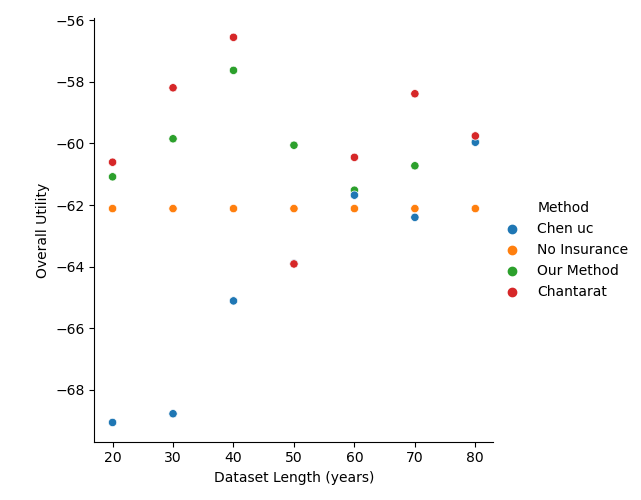
\includegraphics[width=0.75\textwidth]{../../../output/figures/Midwest Evaluation/Midwest_Overall Utility_Length.png}
    \end{figure}
\end{frame}

\begin{frame}{Midwest: Insurer Cost}
    \begin{figure}
        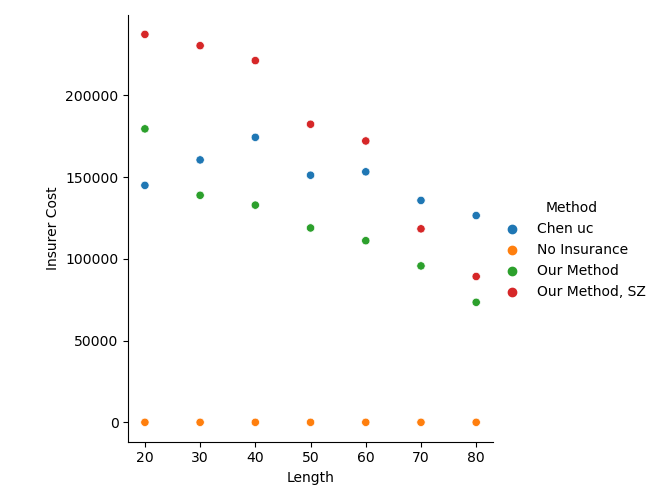
\includegraphics[width=0.75\textwidth]{../../../output/figures/Midwest Evaluation/Midwest_Insurer Cost_Length.png}
    \end{figure}
\end{frame}


\section*{Moving Forward}
\begin{frame}{Things I was thinking about adding}
    \begin{itemize}
        \item Deep dive as to why my method does better, and when it does better?
        \item Run the same evaluation but with shuffled data instead of having it orderd. 
       \item I wanted to do more of a deep dive on the benefits of taking a portfolio approach, but not sure how beyond just looking at capital requirements. Maybe using an expected return and variance approach?
        \item A robustness check on the stability of the solutions at different dataset lengths.
    \end{itemize}
    
\end{frame}

\begin{frame}{Questions}
    \begin{itemize}
        \item What else should I report?
        \item How can I strengthen this evaluation?
       \item Any robustness checks I should add?
        \item I feel like I should do a deep dive as to why the method does
    \end{itemize}
    
\end{frame}

\begin{frame}{Thai Data}
    \begin{itemize}
        \item Plot-level losses caused by natural disasters between 2015-2022. 
        \item I can access the raw data, and they can send me aggregate versions as well. There are around 7000 counties in Thailand, and around 80,000 villages, the data can be aggregated at both of those levels. 
    \end{itemize}
    
\end{frame}

\section*{Implementation Details}
\begin{frame}{Loss Definition}
    From what I can tell from the replication files, they seem to define loss in every year as: 
    \begin{align*}
        \ell_{st} &= R^*_s - R_{st}
    \end{align*}

    where $R^*_s$ is the maximum revenue observed in state $s$ across all time periods, and $R_{st}$ is the revenue in state $s$ at time $t$. 
\end{frame}

\begin{frame}{Initial wealth}
    According to the paper, they set $w_0 = 389$. However, in the replication files, they set it to be $w_0 = 813 - 504 + 389$. According to the comments, $504$ is the fixed cost of operating a farm, and there are no comments regarding the $813$, I'm assuming it corresponds to $R^*$. 
\end{frame}

\begin{frame}{Detrending}
    \begin{itemize}
        \item According to the paper, they detrend the county level yield data using a 2nd order polynomial fit with a ``robust'' regression method, but they don't specify what they use, and it's not in the replication files. They also don't specify if they remove the trend using additive or multiplicative decomposition model. Using an additive decomposition model yielded the most similar losses to what they provide in the replication files. 
        \item There are a couple of papers showing that using locally weighted regression to detrend works better. 
    \end{itemize}
    
\end{frame}

\section*{Questions}
\begin{frame}{Questions}
    \begin{itemize}
        \item Would it make sense to define loss as deviation from historical average? Allowing it to be positive in some years? In other words, we would first adjust all of the yield data to 2020 levels and then calculate the historical average. The loss in each year would be the deviation from this historical average. 
        \item Should I simply follow their lead on detrending? Or should I try to improve on it?
        \item Do you think it's necessary to show results with both definitions of the premium?
        \item Do you think subsidy vs lump sum results would be interesting?
    \end{itemize}
\end{frame}

\section*{Chen Premium Results}
\subsection*{Illinois Results}
\begin{frame}{Their Defn of Premium: Illinois Utility}
    \begin{figure}
        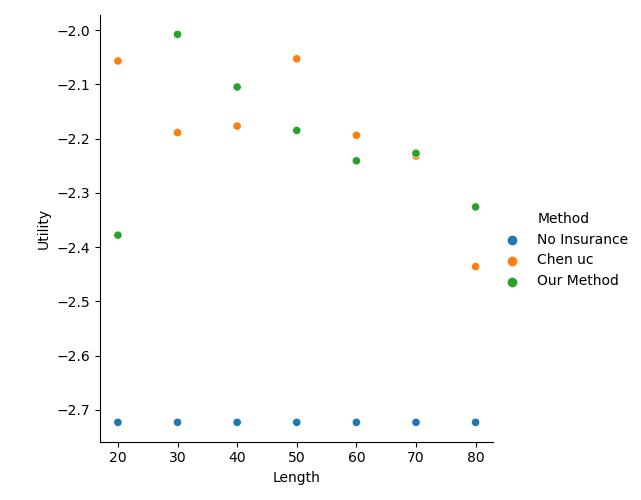
\includegraphics[width=0.75\textwidth]{../../../output/figures/Chen Premium/Illinois_Utility_Length_ml1241.png}
    \end{figure}
\end{frame}

\subsection*{Iowa Results}
\begin{frame}{Their Defn of Premium: Iowa Utility}
    \begin{figure}
        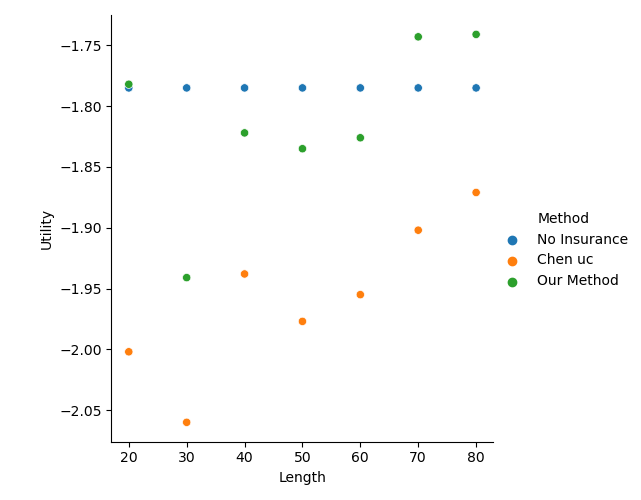
\includegraphics[width=0.75\textwidth]{../../../output/figures/Chen Premium/Iowa_Utility_Length_ml1241.png}
    \end{figure}
\end{frame}

\subsection*{Missouri Results}
\begin{frame}{Their Defn of Premium: Missouri Utility}
    \begin{figure}
        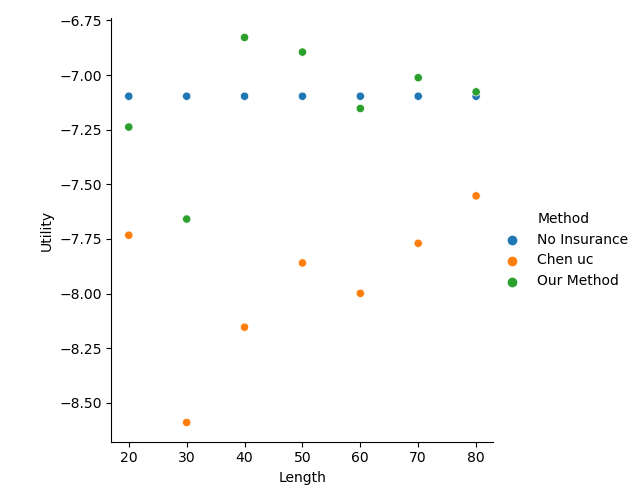
\includegraphics[width=0.75\textwidth]{../../../output/figures/Chen Premium/Missouri_Utility_Length_ml1241.png}
    \end{figure}
\end{frame}

\subsection*{Indiana Results}
\begin{frame}{Their Defn of Premium: Indiana Utility}
    \begin{figure}
        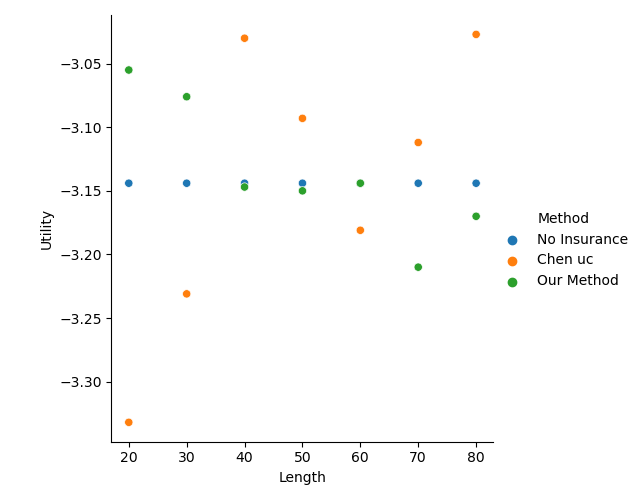
\includegraphics[width=0.75\textwidth]{../../../output/figures/Chen Premium/Indiana_Utility_Length_ml1241.png}
    \end{figure}
\end{frame}



% \section{Conclusion and Next Steps}
% \subsection{Conclusions}
% \begin{frame}{Conclusions}
%     \begin{itemize}
%     \setlength\itemsep{2em}
%         \item The contracts designed by our model are able to offer better protection at a similar costs, or comparable protection at lower costs than the baseline method. 
%         \item It outperforms the baseline when the prediction model is incorrectly specified and on the Kenyan pastoralist data. 
%         \item Our method is more cost effective because it takes into account spatial correlations between  areas and the costs of capital requirements. Thus, the model makes better trade offs between costs and coverage than the baseline method. 
        
%     \end{itemize}
% \end{frame}

% \subsection{Next Steps}
% \begin{frame}{Next Steps}
% \begin{itemize}
% \setlength\itemsep{2em}
%     \item We are working with practitioners to improve the model and possibly test it in practice.
%     \item We are working with the Bank of Thailand on the implementation of their satellite-based index insurance program. 
%     \item We are also talking to the International Research Institute for Climate and Society at Columbia, they have worked on the implementation of numerous index insurance programs in Africa.   
% \end{itemize}
% \end{frame}

\begin{frame}[noframenumbering, plain]{References}
\printbibliography
\end{frame}

\begin{frame}[noframenumbering, plain]{Idealized CVaR Model}
% \label{ideal-model}
\begin{itemize}
    \item \textbf{Objective:} conditional value at risk of the farmers' loss net of insurance.
    \item  \textbf{Constraint 1:} piecewise linear structure of the contract. 
    \item \textbf{Constraint 2:} budget constraint.
    \item \textbf{Constraint 3:} definition of required capital.
\end{itemize}
 
\begin{align}
        \min_{a,b,\pi, K}  & \quad CVaR_{1-\epsilon}\left ( \ell - I(\theta) \right ) \notag\\
        \text{s.t.   }I(\theta) &= \min \{ (a\hat{\ell}(\theta) + b)^+,P \} \\
        \mathbb{E}\left [ I(\theta) \right ] &+ c_{\kappa} K \leq B \\
        K &= \left( CVaR_{1-\epsilon}\left ( I(\theta) \right ) - \mathbb{E}[I(\theta)] \right) \label{cons-budget}
    \end{align}
\end{frame}

\begin{frame}[noframenumbering, plain]{The problem is non-convex, so we need convex approximations}
\label{convex-approx}
We use the following approximations of $I(\theta)$ to make the problem convex: 
\begin{align*}
    \overline{I(\theta)} &\triangleq \max \left \{ 0,a\hat{\ell}(\theta) + b\right \} \\
    \underline{I(\theta)} &\triangleq \min \{ a\hat{\ell}(\theta) + b,K \}
\end{align*}
\begin{itemize}
    \item Note that $\overline{I(\theta)} \geq I(\theta)$ and $\overline{I(\theta)}$ is convex. Conversely, $\underline{I(\theta)} \leq I(\theta)$ and $\underline{I(\theta)}$ is concave. 
    \item We replace $I(\theta)$ with either $\overline{I(\theta)}$ or $\underline{I(\theta)}$ where necessary to obtain conservative and convex approximations. 
    \item We also need approximations or proxies for $E[I(\theta)]$ in constraint . We use $\pi_{SQ} = E[I_{SQ}(\theta)]$, where $I_{SQ}$ is the contract designed using the status quo method, as a proxy for $E[I(\theta)]$ in constraint .
\end{itemize}
\end{frame}



\end{document}